\pagestyle{fancy}
\renewcommand{\theUnit}{2}
\ifthenelse{\isundefined{\UnitPageNumbers}}{}{\setcounter{page}{1}}
\rhead{Chapter \theUnit: Exploratory Data Analysis}
\lhead{Math 3382: Statistical Theory}
%\lhead{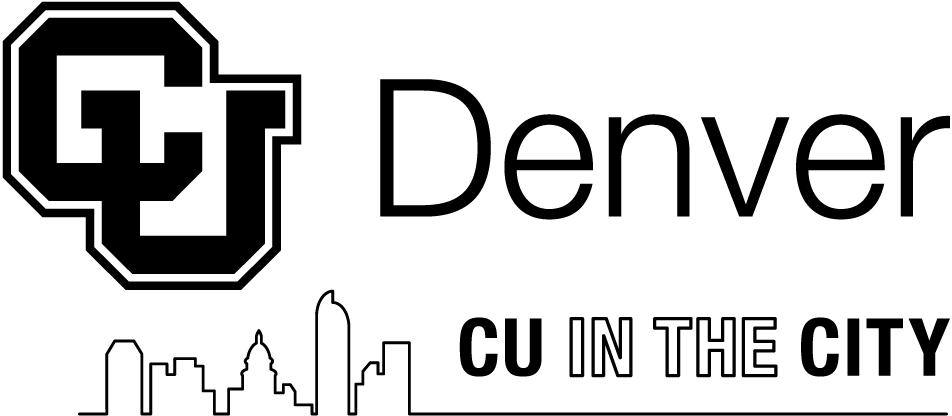
\includegraphics[width=1.25cm]{CUDenver-Logo.png}}
\rfoot{\mypage}
\cfoot{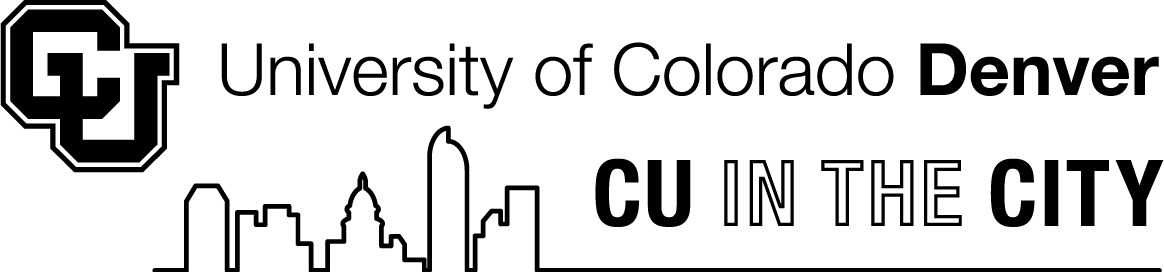
\includegraphics[width=2.25cm]{CUDenver-Logo-coverpage.png}}
\lfoot{Adam Spiegler}
\fancypagestyle{firstfooter}{\footskip = 50pt}
\renewcommand{\footrulewidth}{.4pt}
%%%%%%%%%%%%%%%%%%%%%%%%%%%
\vspace*{-20pt} \thispagestyle{firstfooter}


%\begin{tasks}[counter-format = {(tsk[a])},label-offset = {0.8em},label-format = {\color{black}\bfseries}](2)

\pagebegin{Exploring Data with R and R Studio}

Most of the time this semester, we will be working with very large datasets and/or using simulation based methods that require lots of computations.
 Therefore, we will frequently be using technology as a tool to investigate data and do analysis. Statisticians use different tools (R, Python, Excel, SPSS, STATA, Minitab, SAS and so on!) in different fields. In data science, the two most universal and powerful tools are programming with R and/or Python. This semester, we will be coding in R and using R Studio to interface with R.

\bbox
\textbf{Both R and R Studio are free, open source software and can be installed for free on any platform (Mac, PC, Linux).}
\bb
\ii First install the latest version of R:
\bi
\ii For Windows, go here:   \href{https://cran.r-project.org/bin/windows/base/}{\underline{\colorb{https://cran.r-project.org/bin/windows/base/}}}

\ii For Mac, go here: \href{https://cran.r-project.org/bin/macosx/}{\underline{\colorb{https://cran.r-project.org/bin/macosx/}}}
\ei
\ii Then install the latest version of R Studio. \textbf{\colorr{Choose the Free Open Source License}} here: \href{https://www.rstudio.com/products/rstudio/download/}{\underline{\colorb{https://www.rstudio.com/products/rstudio/download/}}}
\ii Great, you will not need any other technology this semester!
\ee
\ebox

\begin{center}
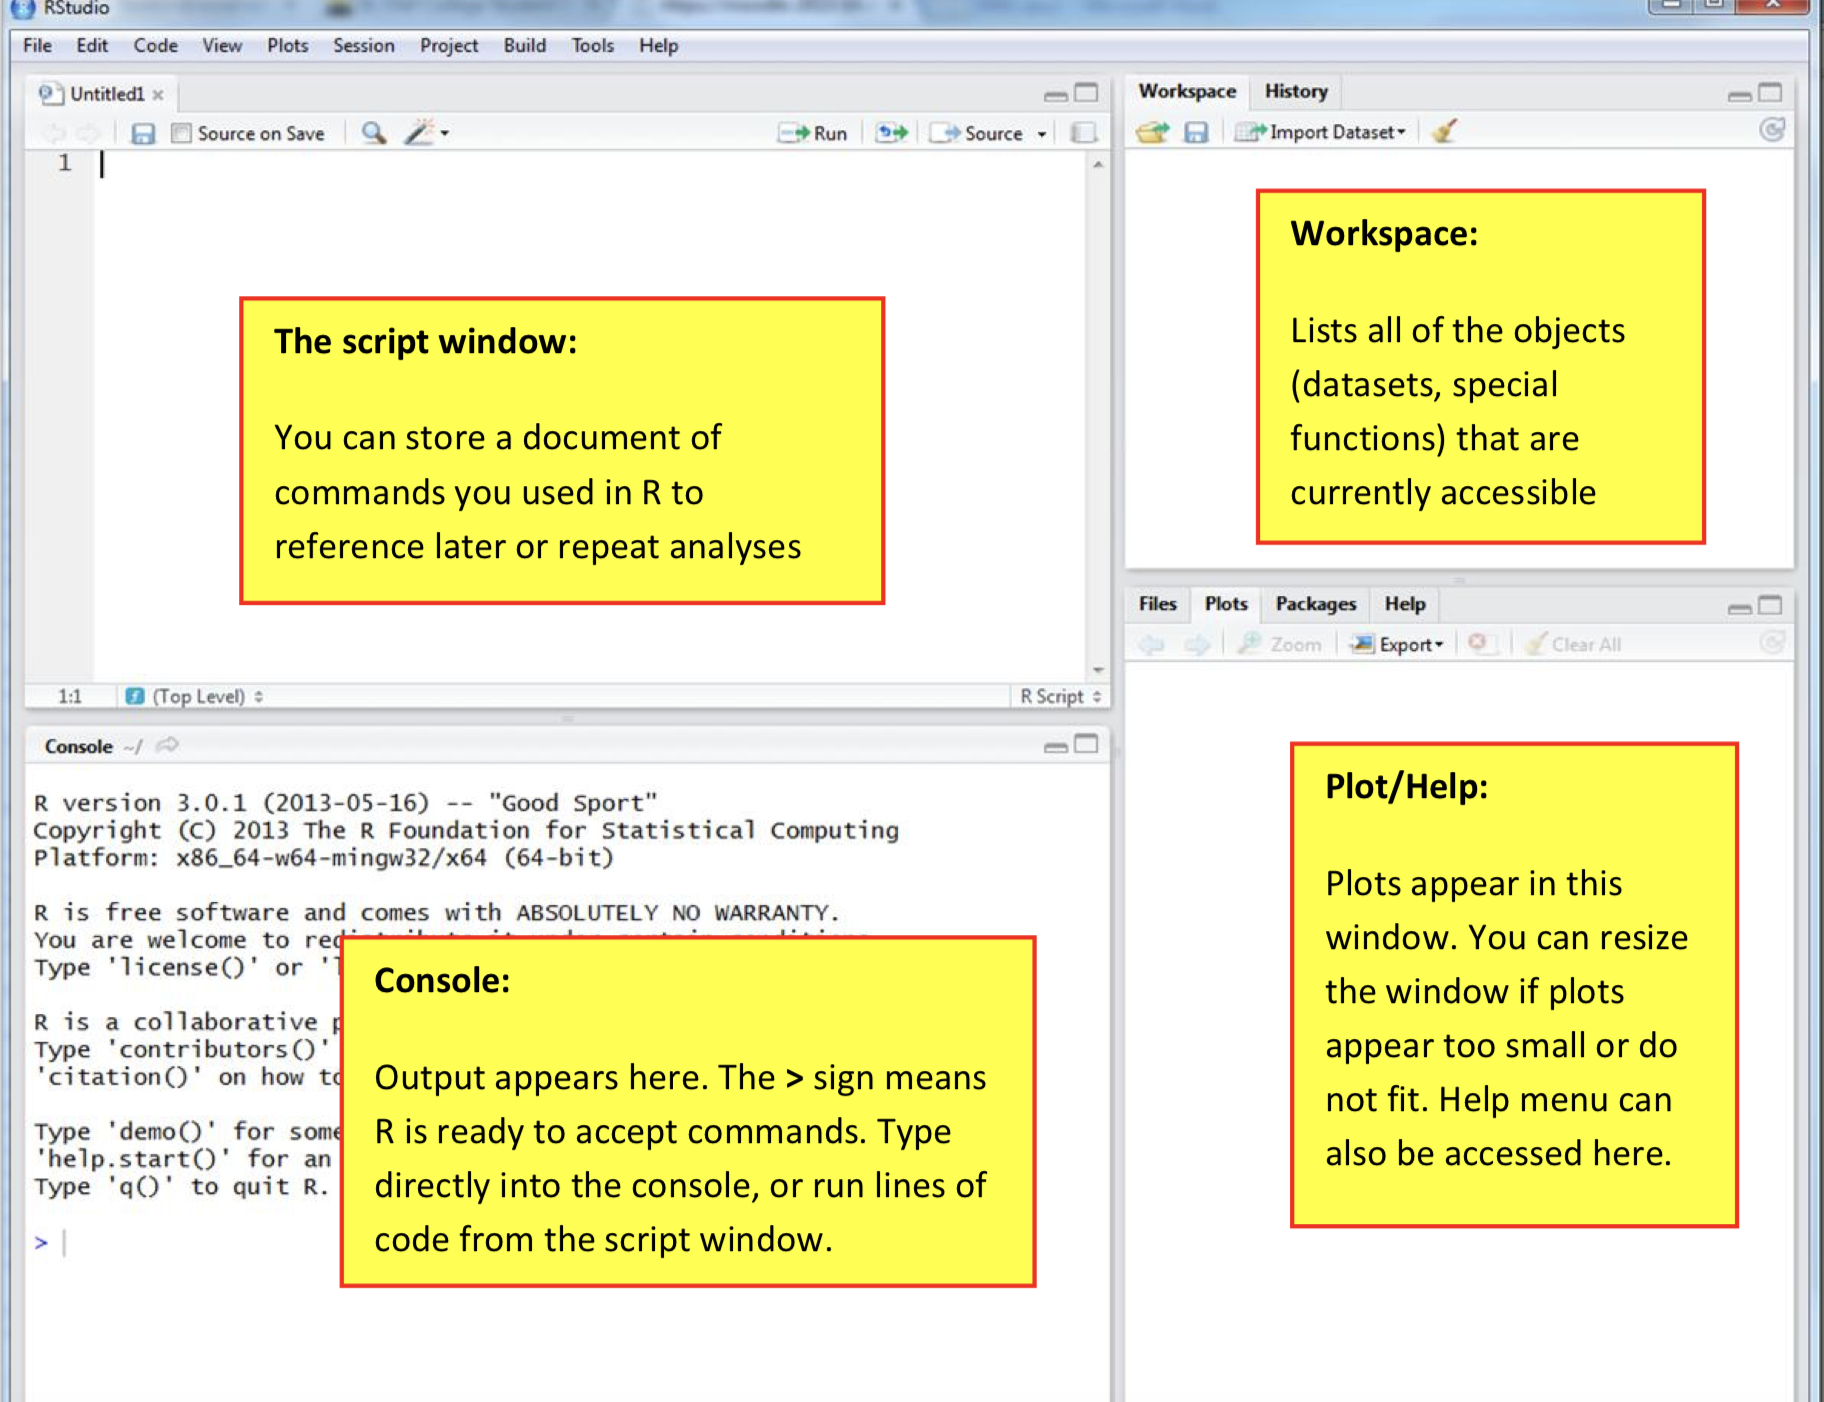
\includegraphics[width=6.25in]{02/R-screen.png}
\end{center}

\clearpage

\pagebegin{What is EDA?}

\bbox
\textbf{\colorb{Exploratory data analysis}}, or EDA for short, can be thought of as a cycle:
\bb
\ii Generate questions about your data.
\ii Search for answers by visualizing, transforming, and modeling your data.
\ii Use what you learn to refine your questions and/or generate new questions.
\ee
\ebox

The main goal of EDA is to develop an understanding of your data.  When you ask a question, the question focuses your attention on a specific part of your dataset and helps you decide which graphs, models, or transformations to make.


\pagebegin{Installing and Loading Packages in R}

To initially install a package, make sure you are connected to the Internet, and enter \\
install.packages(``package\_name'').  You only
need to do this one time; however, each time you want to use a function or dataset from the package, you need to load the package with the command library(package\_name). For now install the following two packages by entering the command

\bbox
\begin{lstlisting}
install.packages(c("tidyverse", "dplyr", "resampledata"))
\end{lstlisting}
\ebox

then load the first two packages by entering \textbf{\colorb{library(tidyverse)}} and then \textbf{\colorb{library(dplyr)}}.

\bigskip

\bbox
Here are some commands for creating commonly used tables and graphics:
\bi
\ii \textbf{\colorb{help(package = "dplyr")}} displays a glossary of all (most?) functions and data in the package dplyr.
\ii \textbf{\colorb{data()}} will list all datasets currently loaded in your R session (across all packages).
\ii \textbf{\colorb{glimpse(dataset\_name)}} gives a glimpse of the dataset.
\ii \textbf{\colorb{view(dataset\_name)}} to view the dataset in tabular form.
\ii \textbf{\colorb{table(categorical\_var\_name)}} creates a frequency table.
%\ii \textbf{\colorb{table(categorical\_var1, categorical\_var2)}} creates a contingency table.
%\ii \textbf{\colorb{prop.table(table\_name)}} creates a joint distribution table.
%\bi 
%\ii[$\circ$]\textbf{\colorb{prop.table(table\_name, 1)}} creates a conditional distribution table so sum across each row equals 1.
%\ii[$\circ$] \textbf{\colorb{prop.table(table\_name, 2)}} creates a conditional distribution table so sum down each column equals 1.
%\ei
\ii \textbf{\colorb{barplot(table\_name, [options])}} creates a bar chart.
%\ii \textbf{\colorb{boxplot(numerical\_variable\_name, [options])}} creates a box plot.
\ei
\ebox

\bb
\ii The package \textbf{dplyr} contains many datasets, one of which is \textbf{\colorg{storms}} . How many observations are in  \textbf{\colorg{storms}}? How many variables? Which variables are numerical and which are categorical? What R code did you use to gain this insight?

\begin{multicols}{2}

\begin{lstlisting}
> glimpse(storms)
\end{lstlisting}

or

\begin{lstlisting}
> view(storms)
\end{lstlisting}

\columnbreak

\small{\colorr{There are 10,010 observations. 13 variables in total. The variables name, status and  category are categorical. The variables year, month, day, hour, lat, long, wind, pressure, ts\_diameter and hu\_diameter.}}

\end{multicols}

\clearpage

\pagebegin{Displaying Categorical Variables: Bar Plots}

\ii Let's explore the following question: ``Which storm types occurred most frequently over the period from 1975 to 2015?''
\bb
\ii Create a frequency table to identify how many storms there are in each \textbf{\colorr{status}}. Write the R code below. 

\begin{multicols}{2}

\begin{lstlisting}
table(storms$status)
\end{lstlisting}

\columnbreak

\begin{tabular}{ccc}
hurricane & tropical depression   &   tropical storm \\
 3091 &  2545  &  4374
 \end{tabular}

\end{multicols}

\ii  Write R code below to create a bar graph to visually present the table. 

\begin{lstlisting}
> types <- table(storms$status)
> barplot(types)
\end{lstlisting}

\begin{multicols}{2}

\columnbreak

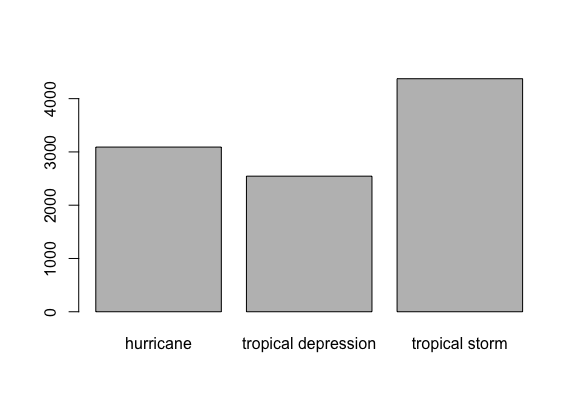
\includegraphics[width=0.4\tw]{02/fig-storm-types.png}

\end{multicols}


\ee
\ee

\bbox
\bi
\ii To refer to values of the  variable \textbf{\colorr{status}} in the dataset  \textbf{\colorg{storms}} , we enter \textbf{\colorg{storms}\$\colorr{status}}.
\ii To perform future manipulations with the output from the table, we can assign this output  to an object called \textbf{types}: 
\begin{lstlisting}
types <- table(storms$status)
\end{lstlisting}
\ii Curious about how to make your barplot prettier? Enter \textbf{\colorb{?barplot}} to view the help documentation for the function barplot.
\ei
\ebox

The variable \textbf{\colorr{status}} in the dataset  \textbf{\colorg{storms}}  is a categorical variable, so we can count how many or what proportion of the observations fall into each classification. There is not a natural notion for the average value of the variable status is. The type of analysis and visualizations we can use depend on what type of data we have. We will revisit categorical data shortly, but for now we will focus on how we summarize and present numerical variables.

\clearpage

\pagebegin{Displaying Numerical Variables: Histograms}

\bbox
A \textbf{\colorb{histogram}} is special bar chart we use to display the distribution of values for a numerical variable.
\bi
\ii Values of the numerical variable are measured on the horizontal axis.
\ii The height of each bar gives the total number of observations in the dataset (called the \textbf{\colorb{frequency}}) in the specified \textbf{\colorb{bin range}}. 
\ii There are no gaps between bars. Empty space means no values are in that bin range.
\ii The R function \textbf{\colorb{hist(numerical\_variable\_name, [options])}} creates a histogram.
\ei
\ebox

 The R code below generates the histogram on the left. Notice there are lots of ways to customize your plots.

\begin{multicols}{2}

\begin{lstlisting}
hist(storms$wind, breaks = 15,
     main = "Distribution of Windspeed from 1975-2015",
     xlab="Wind speed (in knots)",
     xlim = c(0, 160), ylim = c(0,2500), 
     col = "steelblue")
\end{lstlisting}

\columnbreak

\ \vspace{0.35in}

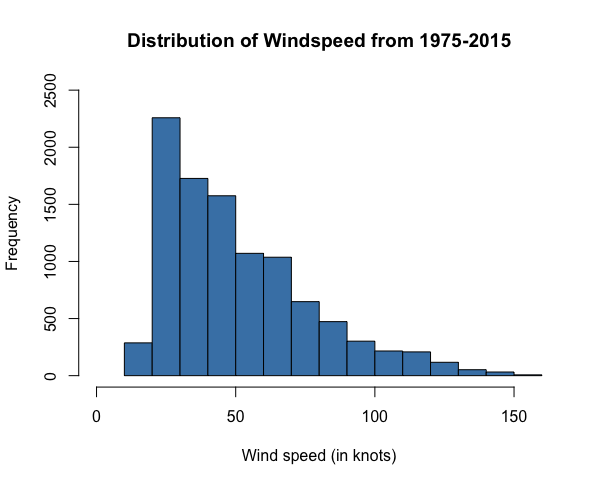
\includegraphics[width=0.4\tw]{02/fig-wind-hist.png}

\end{multicols}

\bb[resume]
\ii How would you describe the shape of the distribution of wind speed shown in the histogram above?

\colorr{It has a tail of outliers off to the left.}

\bigskip

\ii Using R, create a histogram to display the variable \textbf{\colorg{month}}. What does the shape of that graph tell you?  

\begin{multicols}{2}

\begin{lstlisting}
hist(storms$month, 
     breaks = 12, 
     xlab="Month",
     xlim = c(1, 12), 
     ylim = c(0,4500), 
     col = "green",
     main = "Distribution of Storms by Month",
     xaxt='n')
axis(1, at=seq(1, 12, 1), pos=0)
\end{lstlisting}

\columnbreak

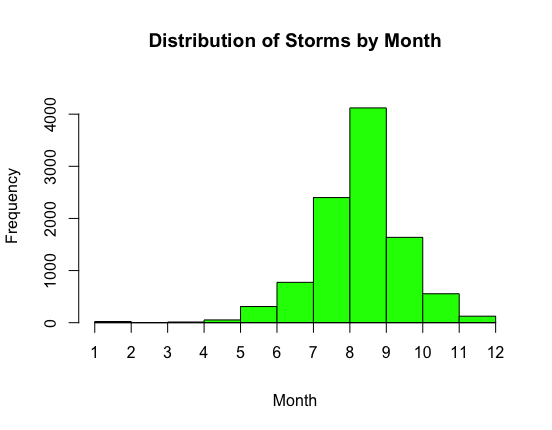
\includegraphics[width=0.3\tw]{02/fig-month-hist.png}

\end{multicols}

\colorr{Most storms occurred in the second half of the year, particular in the months from July-September. There are a few outliers for storms that occurred in the winter, giving a tail to the right.}

\ii Using R, create a histogram to display the variable \textbf{\colorr{long}}. What does the shape of that graph tell you? 

\begin{multicols}{2}

\begin{lstlisting}
hist(storms$long, 
     breaks = 15, 
     xlab="Degrees of Longitude",
     xlim = c(-120, 0), 
     ylim = c(0,1000), 
     col = "red",
     main = "Distribution of Storms by Longitude",
     xaxt='n')
axis(1, at=seq(-120, 0, 10), pos=0)
\end{lstlisting}

\columnbreak

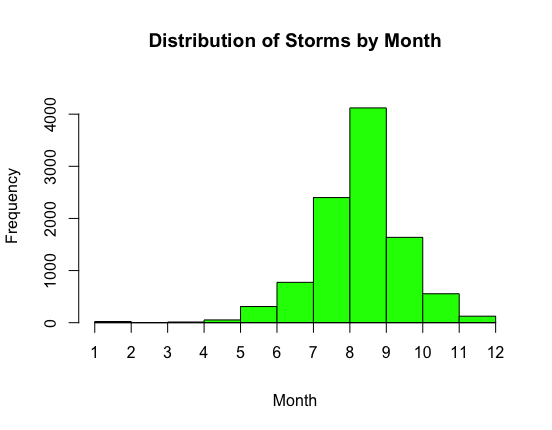
\includegraphics[width=0.3\tw]{02/fig-month-hist.png}

\end{multicols}

\colorr{Most storms occurred between $-100$ and $-30$ degrees longitude. As you move away from the center of the histogram (which is approximately $-65$ degrees longitude), the number of storms that occur goes down as you move further and further to the left or right. The storms are distributed pretty similarly on the left and right side of the center, so the histogram appears to be approximately symmetric.}

\begin{center}
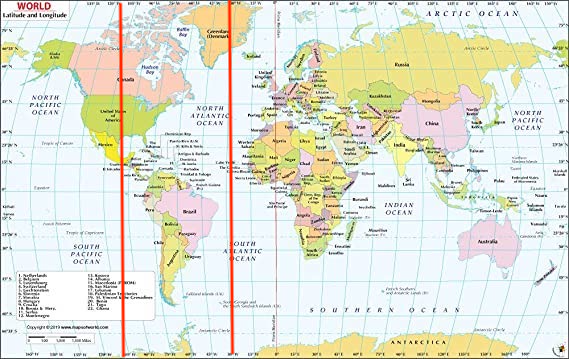
\includegraphics[width=0.8\tw]{02/fig-world-map.png}
\end{center}


\ee

\clearpage

\pagebegin{The Shape of Data}

\bbox
\begin{center}
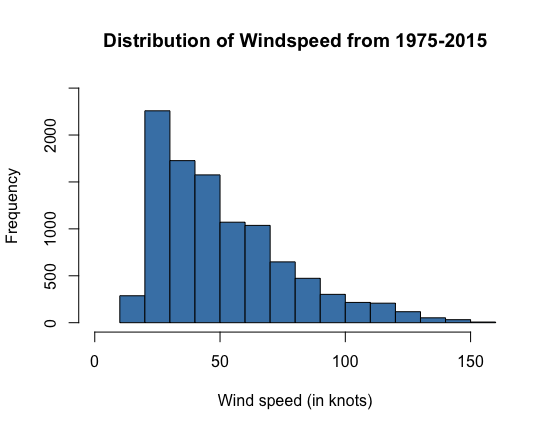
\includegraphics[width=0.3\tw]{02/fig-windspeed-hist.png}
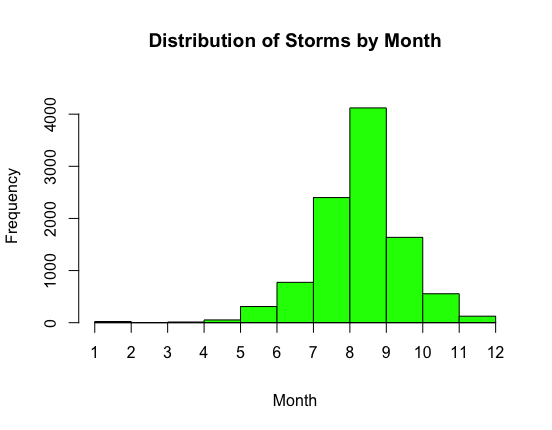
\includegraphics[width=0.3\tw]{02/fig-month-hist.png}
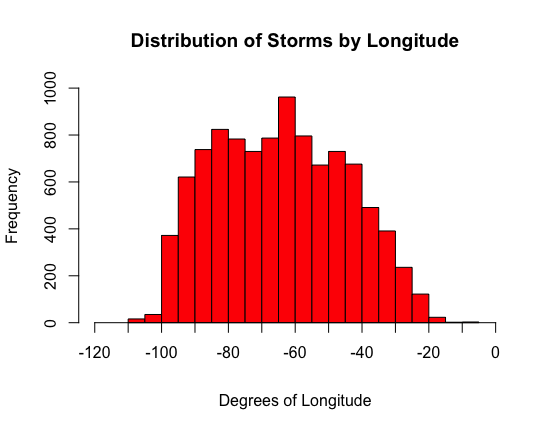
\includegraphics[width=0.3\tw]{02/fig-long-hist.png} 
\end{center}

\bi
\ii The distribution of wind speeds is \alert{skewed right}.
\ii The distribution of months is \alert{skewed left}.
\ii The distribution of longitude is approximately \alert{symmetric}.
\ei
\ebox


\pagebegin{2.2: Measurements of Center}

\bbox
Typical measurements of center are:
\bi
\ii The \alert{mean} is the average. In R, \alert{mean(variable\_name)}
\bi
\ii[$\circ$] We use \colorr{$\mathbf{\bar{x}}$} (pronounced x-bar) to denote a \textbf{\colorr{sample}} mean.
\ii[$\circ$] We use \colorg{$\mathbf{\mu}$} (Greek letter mu) to denote a  \textbf{\colorg{population}} mean.
\ei
\ii The \alert{median} is the $50^{\mbox{th}}$ percentile. 50\% of the values in the dataset are less than the median.  In R, \alert{median(variable\_name)}
\ei
\ebox

\bb[resume]
\ii Compute the mean wind speed of all storms and the median wind speed of all storms. Interpret in practical terms what each tells us. 

\bigskip
%%%%%%%%%%%
%%% Solution below
%%%%%%%%%%
\begin{lstlisting}
mean(storms$wind)  #Mean is 53.495
median(storms$wind) #Median is 45
\end{lstlisting}

\vfill

\ii Why do you think the mean wind speed is greater than the median wind speed of all storms?

\colorr{Because there are some outliers of storms that had very large wind speeds, that will affect the mean more so than the median, so the mean gets pulled over to the right because of the tail in the histogram goes to the right.}

\vfill

\ee

\clearpage

\bbox
\begin{center}
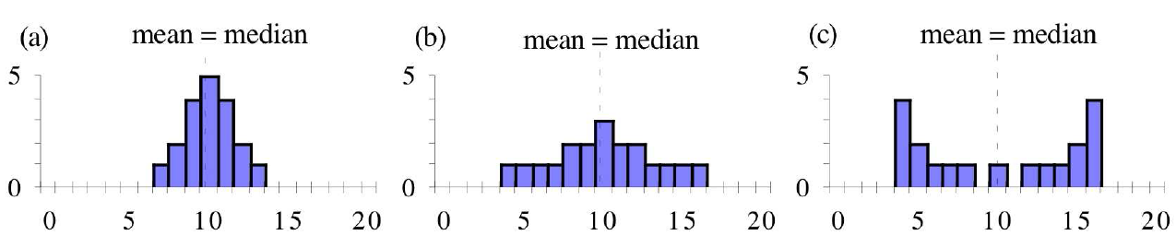
\includegraphics[width=0.75\tw]{02/fig-symmetric.png} \\
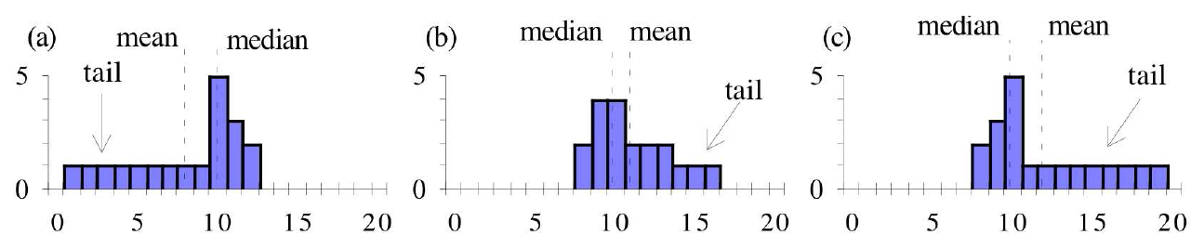
\includegraphics[width=0.75\tw]{02/fig-skewed.png} 
\end{center}

\bi
\ii If the shape of the histogram is \textbf{\colorr{symmetric}}, then the \textbf{\colorr{mean is equal to the median}}.
\ii If the shape of a histogram is \textbf{\colorg{skewed to the left}}, the \textbf{\colorg{mean is less than the median}}.
\ii If the shape of a histogram is \alert{skewed to the right}, the \alert{mean is greater than the median}.
\ei
\ebox

\pagebegin{Filtering and Subsetting Data}

We have seen that the most frequent month is August, followed by July as the second most frequent month. How can we compare the strength of storms that occur in July to August?

\bbox
Here are two useful commands for filtering out a subset of all observations based on some additional condition(s):
\bi
\ii One way to  \textbf{\textcolor{red}{filter}} out the storms that occurred in July:

\begin{lstlisting}
july <- filter(storms, month == "7")
\end{lstlisting}


\ii Or we can \textbf{\textcolor{blue}{subset}} the data with the following command:

\begin{lstlisting}
#keeps all variables, same as filter above
july <- subset(storms, month == "7")
#keeps only windspeed variable
july.wind <- subset(storms, select = wind, month == "7")
#data vector instead of data frame
july.wind.vec <- subset(storms, select = wind, month == "7", drop = T) 
\end{lstlisting}

\ei

\ebox

\bb[resume]
\ii Compute the mean and median wind speed of all storms in July. Compare the values of the mean and median. What does this tell us about the shape of the data?

\begin{lstlisting}
july <- filter(storms, month == "7")
mean(july$wind)   # mean is 41.195 knots
median(july$wind) # median is 37.5 knots
\end{lstlisting}

\colorr{Since the mean is greater than the median, the data is skewed to the right.}

\clearpage


\ii In which month are the storms more severe? What statistics did you use to draw your conclusion?

\colorr{Similarly filtering the data for August and September we can calculate the mean wind speed for each month:}

\begin{lstlisting}
july <- filter(storms, month == "7")
aug <- filter(storms, month == "8")
sep <- filter(storms, month == "9")

mean(july$wind) # mean is 41.195 knots
mean(aug$wind) # mean is 52.1 knots
mean(sep$wind) # mean is 57.958 knots
\end{lstlisting}

\colorr{We see the storms in September have on average the greatest wind speed.}

\ee

\clearpage

\pagebegin{2.2 Measurements of Spread}

\bbox
Typical measurements of spread are:
\bi
\ii The \alert{range} $= \mbox{max} - \mbox{min}$.
\ii The \alert{standard deviation} approximately measures the average distance of each value from the mean value. 
\bi
\ii[$\circ$] For a sample, $\dsty s = \sqrt{\frac{\sum_{i=1}^{n} (x_i - \bar{x})^2}{n-1}}$.
\ii[$\circ$] In R, \alert{sd(var\_name)}
\ii[$\circ$] We use \colorr{$\mathbf{s}$}  to denote a \textbf{\colorr{sample}} standard deviation.
\ii[$\circ$] We use \colorg{$\mathbf{\sigma}$} (Greek letter sigma) to denote a  \textbf{\colorg{population}} standard deviation.
\ei
\ei
\ebox

\begin{center}
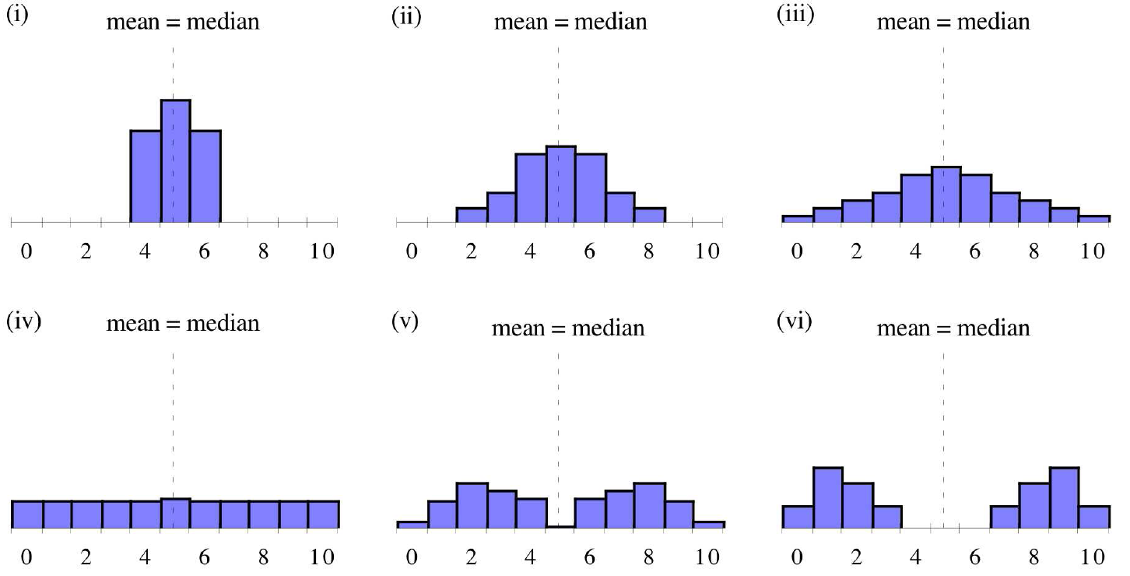
\includegraphics[width=0.75\tw]{02/fig-compare-sd.png}
\end{center}

\bb[resume]
\ii Which of the histograms (i)-(vi) has the largest range? The smallest range?

\colorr{Histograms (iii), (iv), (v), and (vi) all have the same range, namely 10.}

\vfill

\ii Which of the histograms (i)-(vi) has the largest standard deviation? The smallest standard deviation?


\colorr{Histograms (vi) has the greatest standard deviation. Histogram (i) has the smallest standard deviation.}

\vfill
\ee

\clearpage

\pagebegin{Quantiles}

\bbox
\bi
\ii  The $25^{\mbox{th}}$ percentile (\alert{first quartile}) is denoted $\mathbf{Q_1}$.  In R, \alert{quantile(var\_name, probs = $0.25$)}
\ii  The $75^{\mbox{th}}$ percentile (\textbf{\colorr{third quartile}}) is denoted $\mathbf{Q_3}$.  In R,\\ \textbf{\colorr{quantile(var\_name, probs = $0.75$)}}
 \ii The \textbf{\colorg{Interquartile Range (IQR)}}$=Q_3-Q_1$. In R, \textbf{\colorg{IQR(var\_name)}}
\ii The \alert{five number summary} can also provide a good description of the spread of the values since we know 25\% of the values
in a dataset fall between each consecutive pair of values:
\[  \alert{(\mbox{min}, Q_1 , \mbox{median}, Q_3, \mbox{max} )} \]
 In R, \alert{summary(var\_name)}
\ei
\ebox

\bb[resume]
\ii Give the five number summary for the wind speed of all storms in July.  What R code did you use?


\begin{multicols}{2}

\begin{lstlisting}
summary(july$wind)
\end{lstlisting}

\columnbreak

\begin{tabular}{cccccc}
Min. & 1st Qu.  & Median   & Mean & 3rd Qu. &   Max.\\ 
$10.0$ & $30.0$ &  $37.5$  & $41.2$  & $50.0$  & $140.0$
\end{tabular}

\end{multicols}

\colorr{Thus we see the five number summary is $(10, 30, 37.5, 50, 140)$.}

\ee

\pagebegin{2.3: Boxplots and Five Number Summaries}

The five number summary for August wind speeds is $(10, 30, 45, 65, 150)$. Below is a \textbf{boxplot} for
this data generated with the following code:



\begin{multicols}{2}

\begin{lstlisting}
boxplot(aug$wind, 
        main = "August Windspeeds", 
        horizontal = FALSE)
\end{lstlisting}
%boxplot(AA$\$$FlightLength,\\
%$\mbox{ }$ \hspace{0.25in}   main = ``American Airline Flight Lengths'', \\
%$\mbox{ }$ \hspace{0.25in}    horizontal = FALSE)

\columnbreak

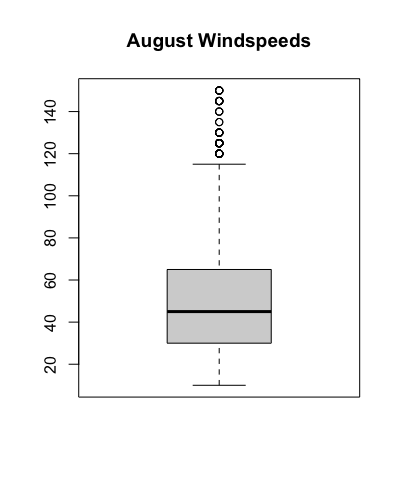
\includegraphics[width=0.45\tw]{02/fig-aug-box.png}

\end{multicols}

\clearpage



\bb[resume]
\ii Create a boxplot to illustrate the distribution of windspeeds of July storms. What code did you use?  \vfill

%%%%%%%%%%%
%%% Solution below
%%%%%%%%%%

\begin{multicols}{2}

\begin{lstlisting}
boxplot(july$wind, 
        main = "July windspeeds", 
        horizontal = TRUE)
\end{lstlisting}

\columnbreak

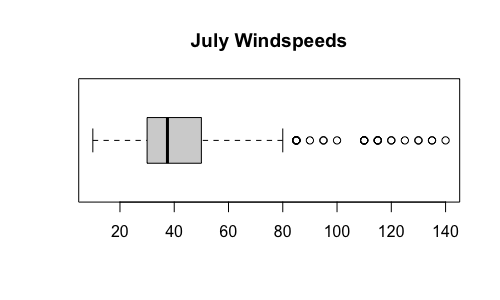
\includegraphics[width=0.45\tw]{02/fig-july-box.png}

\end{multicols}

\ii Create a side by side box plot to compare the distribution of wind speeds between July and August. Write your code below. \vfill

%%%%%%%%%%%
%%% Solution below
%%%%%%%%%%
\begin{multicols}{2}

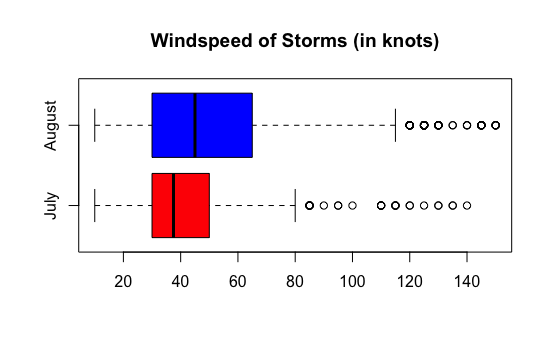
\includegraphics[width=0.45\tw]{02/fig-sidebyside.png}

\columnbreak

\begin{lstlisting}
boxplot(july$wind, aug$wind, 
        main = "Windspeed of Storms (knots)", 
        names = c("July", "August"), 
        col = c("red", "blue"), 
        horizontal = TRUE)
\end{lstlisting}

\end{multicols}


\ee

\bbox
To create a boxplot:
\bi
\ii Find the values of $Q_1$, median, and $Q_3$.
\ii Draw a box with bottom edges at $Q_1$ and $Q_2$ and line inside the box for the median.
\ii Identify the upper and lower fence:
\bi
\ii[$\circ$] Upper fence $=Q_3 + 1.5(\mbox{IQR})$.
\ii[$\circ$] Lower fence $=Q_1 - 1.5(\mbox{IQR})$.
\ei
\ii Extend whiskers from the lower edge to the smallest observation greater than the lower fence, and from the upper
edge to the largest value that is less than the upper fence.
\ii The observations that are less than the lower fence or greater than the upper fence are considered \alert{outliers}. These values are marked by individual points.
\ei
\ebox

